\chapter{Stand van zaken}
\label{ch:stand-van-zaken}

% Tip: Begin elk hoofdstuk met een paragraaf inleiding die beschrijft hoe
% dit hoofdstuk past binnen het geheel van de bachelorproef. Geef in het
% bijzonder aan wat de link is met het vorige en volgende hoofdstuk.

% Pas na deze inleidende paragraaf komt de eerste sectiehoofding.


Voordat de bachelorproef van start kan gaan,is het belangrijk om inzicht te 
krijgen in de basis van mobiele applicaties en hoe dat ze precies ontwikkeld worden. 
Pas na deze uitleg kan het onderzoek worden uitgevoerd. Eerst worden mobiele applicaties 
algemeen uitgelegd alsook de verschillende soorten mobiele applicaties. 
Daarna worden de ontwikkelmethodes en hun verschillen uitgelegd die gebruikt worden tijdens het 
onderzoek.

\section{Inleiding mobiele applicatie-ontwikkeling}

De ontwikkeling van mobiele applicaties is het proces waarbij er software wordt 
gemaakt voor smartphones, tablets, televisies en digitale assistenten \autocite{Palko2021}. 
Deze applicaties worden ontwikkeld voor de besturingssystemen Android en IOS. 
De software kan op verschillende manieren op een apparaat komen. Het kan gedownload 
worden uit een app store, vooraf op het apparaat worden geïnstalleerd of het kan worden 
geopend via een mobiele webbrowser \autocite{IBM2023}. 
\\\\
Mobiele applicaties worden in veel sectoren gebruikt zoals: telecommunicatie, 
e-commerce, verzekeringen, gezondheidszorg, overheid, enz. Ze worden in deze sectoren 
veel gebruikt omdat het een makkelijke en populaire manier is om mensen en bedrijven in contact te brengen 
met elkaar en met het internet. Op deze manier kunnen bedrijven relevant, responsief 
en succesvol blijven. 
\\\\
Er bestaan verschillende soorten mobiele applicaties, zoals native, web en hybride 
applicaties \autocite{AWS2023}. Elke soort mobiele applicatie is een manier waarop dat 
applicaties op smartphones of computers worden geïnstalleerd of werken.

\subsection{Native applicaties}\label{ch:native-applicaties}
Dit is de meest gekende en gebruikte soort mobiele applicaties. Hierbij wordt een applicatie 
gedownload en geïnstalleerd op een apparaat. Het is een applicatie die specifiek wordt ontwikkeld 
voor één besturingssysteem, zoals Android of IOS \autocite{Laarhoven2021}. Native applicaties 
zijn vaak sneller en gebruiksvriendelijker dan een web of hybride applicatie. Dit komt omdat 
de applicaties platformspecifieke software gebruiken. 

\subsubsection{Voordelen van native applicaties}
\label{ch:voordelen-native-applicaties}
\paragraph{Platformspecifieke code}
Omdat er platformspecifieke code wordt gebruikt, heeft de applicatie direct toegang tot 
de interne APIs van een apparaat \autocite{AWS2023}. Hierdoor zal ook de performantie hoger 
liggen dan bij web of hybride applicaties. Ook hebben ze daardoor direct toegang tot bepaalde 
functionaliteiten zoals: camera, gps, versnellingsmeter, kompas, lijst van contacten, enz. 
Daarnaast hebben ze ook toegang tot het notificatiesysteem en werken ze offline in tegenstelling 
tot web applicaties \autocite{Budiu2016}. 

\paragraph{Fouten vermijden of oplossen}
Omdat het niet nodig is om twee applicaties te onderhouden vanuit één \gls{codebase}, kan 
het makkelijker zijn om fouten bij een bepaald platform op de sporen of compleet te 
vermijden \autocite{Koffer2023}. 

\paragraph{User interface}
Nog een ander voordeel van platformspecifieke code en het gebruik van interne APIs is de UI. 
Omdat de applicatie gebruik maakt van de interne APIs zal de UI consistenter zijn. 
Dit zal voor een betere gebruikerservaring zorgen aangezien dat de applicatie gebruiksvriendelijker 
aanvoelt \autocite{Kotlin2023}. 

\paragraph{App store ondersteuning}
Dankzij hun betere performantie en snelheid zullen native applicaties populairder zijn in de app store. 
Het is ook makkelijker om native applicaties te publiceren in de app store \autocite{Koffer2023}.

\subsubsection{Nadelen van native applicaties}
\paragraph{Kost en onderhoudsprijs}
Aangezien dat er een applicatie ontwikkeld wordt voor twee platformen, zal de kostprijs en 
ontwikkeltijd van een applicatie hoger liggen dan als er één applicatie ontwikkeld moet 
worden. Daarnaast moeten beide applicaties worden onderhouden na dat ze 
ontwikkeld zijn. Het is dus niet enkel de kostprijs die hoger zal zijn. Ook de onderhoudsprijs zal 
hoger liggen \autocite{AWS2023}. 

\paragraph{Verschillende logica}
Door dat de applicatie twee keer ontwikkeld wordt, is het mogelijk dat de business 
logica op bepaalde plaatsen in de applicatie verschillend is van elkaar. 
Er moet dus altijd aandachtig getest worden zodat dit niet het geval is \autocite{Kotlin2023}.

\paragraph{Downloaden}
Zoals eerder gezegd, wordt de applicatie gedownload van op een app store \ref{ch:native-applicaties}. 
Om die download te doen is er een internetverbinding nodig, 
pas daarna kan de applicatie indien mogelijk offline werken.

\subsection{Web applicaties}
Web applicaties zijn niet echt applicaties maar het zijn mobiele versies van responsive websites. 
Een web applicatie simuleert een native applicatie en wordt niet geïnstalleerd op een 
apparaat \autocite{Beeproger2023}. Ze zullen dus net zoals bij websites een HTTP request naar 
een server sturen die op zijn beurt dan een HTTP response zal terugsturen.
\begin{figure}[H]
    \centering
    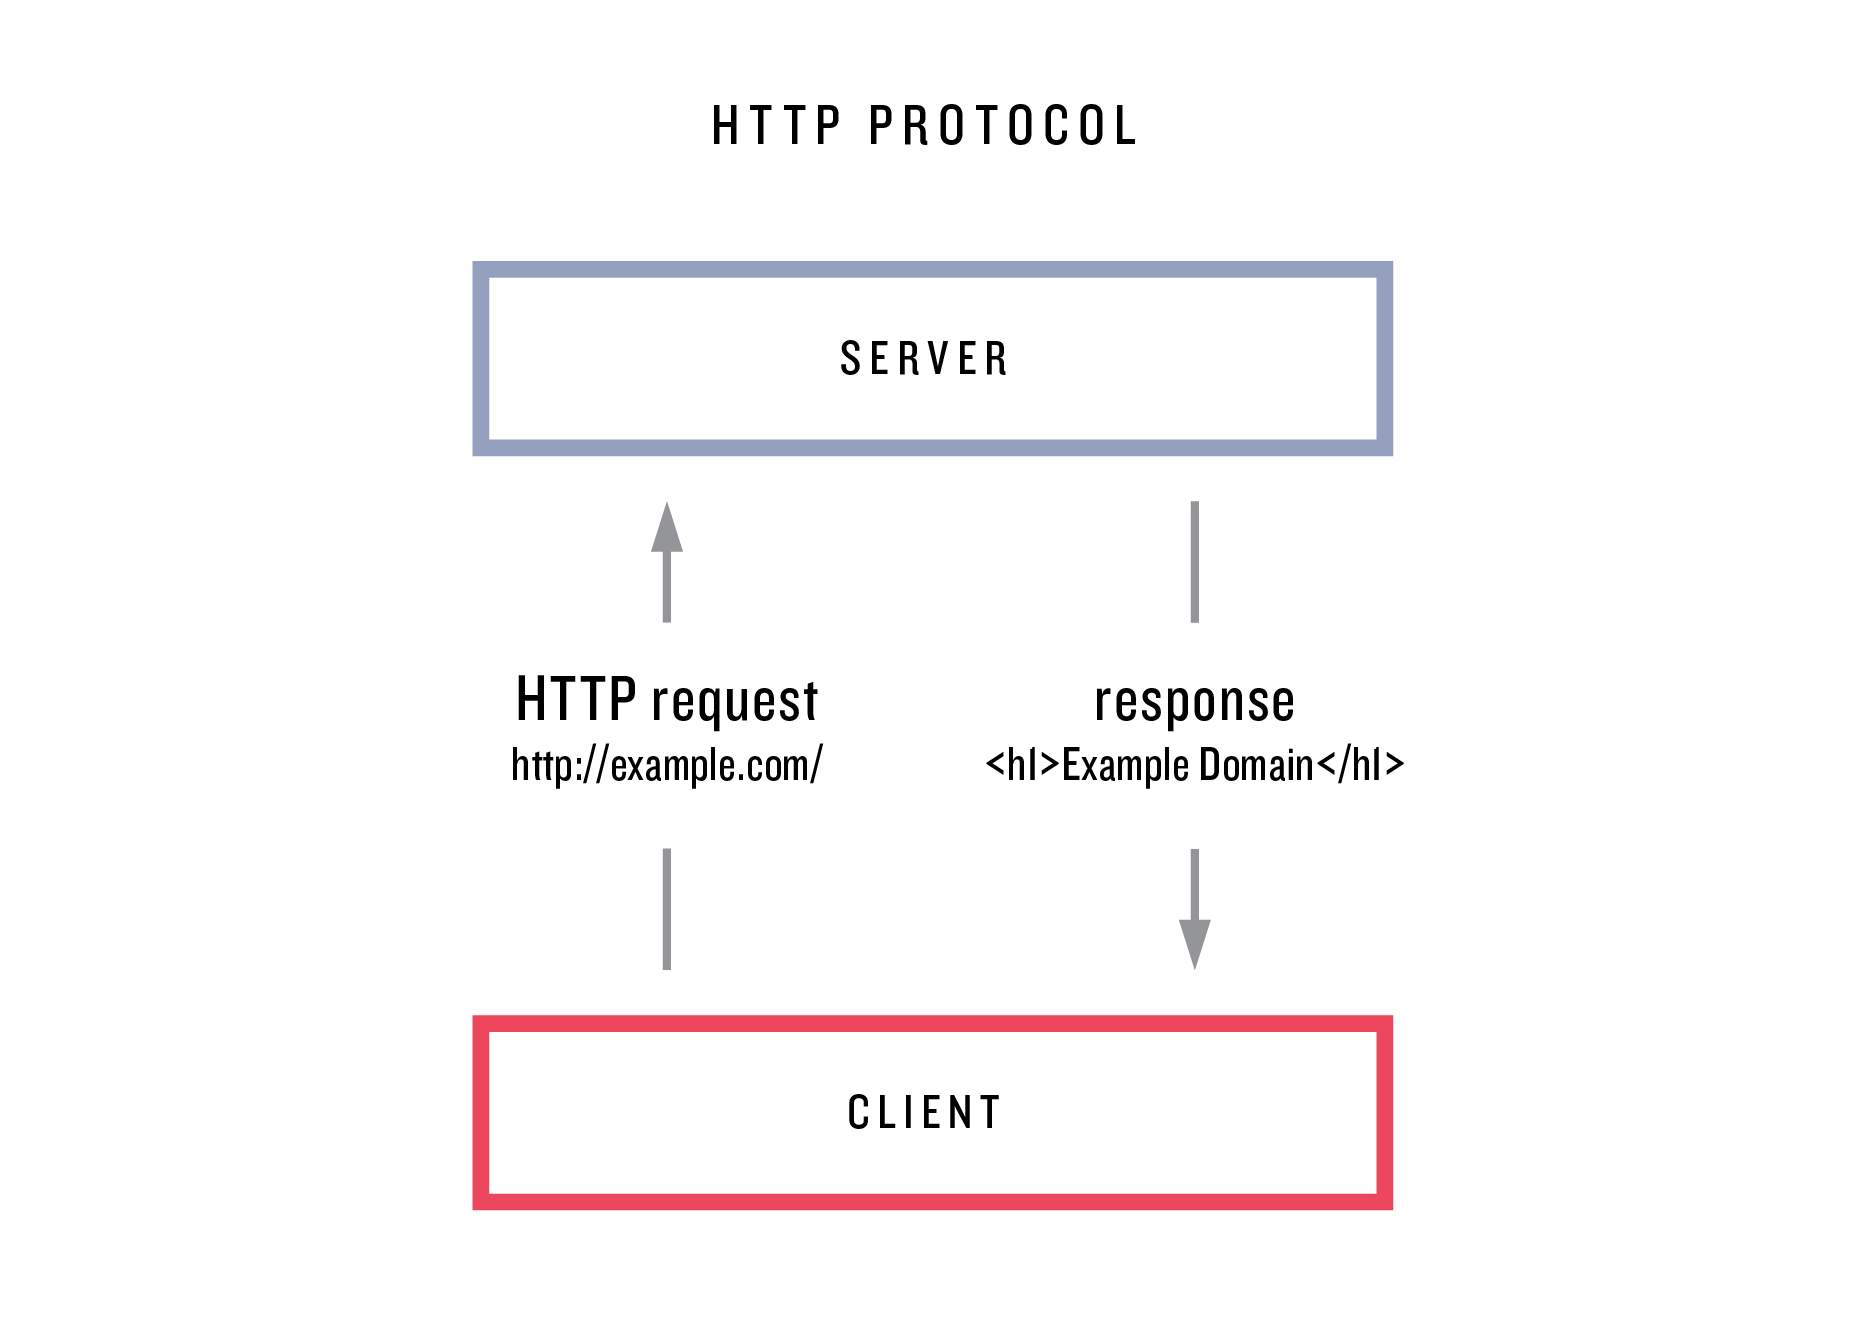
\includegraphics[height=0.4\textheight]{httpprotocol.png}
    \caption{Request-response cycle van HyperText Transfer Protocol \parencite{Hartl2019}.}
\end{figure}
Aangezien dat web applicaties niet geïnstalleerd worden is het dus wel nodig om een internetverbinding 
te hebben bij het gebruik er van. Ze worden vaak gebruikt door bedrijven om informatie en diensten 
aan hun klanten op een veilige manier aan te bieden \autocite{Nehra2023}. 
\\\\
Een web applicatie is bereikbaar door een unieke URL in te voeren in een browser 
\autocite{Beeproger2023}. Microsoft Word is een voorbeeld van een native applicatie die 
gebruikers moeten installeren op hun apparaat, in vergelijking met Google Docs dat een web applicatie 
is en dat niet geïnstalleerd moet worden \autocite{Nehra2023}.
\\\\
Web applicaties worden op dezelfde manier gemaakt als websites. Ze maken gebruik van HTML, CSS en JavaScript. 
De meeste web applicaties gebruiken een web server voor het verwerken en beheren van requests, een 
applicatieserver om de gevraagde taken te voltooien en een database om de gevraagde data 
op te halen \autocite{Varsha2023}.

\subsubsection{Voordelen van web applicaties}\label{ch:VoordelenWebApplicaties}
\paragraph{Kostprijs}
Aangezien dat één web applicatie op alle platformen draait zal dit veel goedkoper uitkomen dan bij native 
applicaties \autocite{Laarhoven2021}. Er moet namelijk maar één applicatie ontwikkeld worden die op alle 
platformen zal draaien

\paragraph{Updates}
Omdat web applicaties aan een URL gelinkt zijn, is het makkelijk om updates uit te voeren op de applicatie. 
De URL wordt vanzelf periodiek geüpdatet. Hierdoor wordt de applicatie automatisch ook up to date gehouden 
ongeacht van het platform dat een gebruiker gebruikt \autocite{Varsha2023}.

\paragraph{Installatie \& Compatibiliteit}
Daarnaast zoals gezegd, moet een web applicatie niet geïnstalleerd worden. Ze is beschikbaar op alle 
platformen en browsers. Waardoor ze zeer toegankelijk is voor gebruikers. Er is enkel een actieve 
internetverbinding nodig.

\paragraph{Integratie}
Web applicaties hebben daarnaast ook nog de mogelijkheid om makkelijk met andere web applicaties te integreren. 
Ze kunnen bijvoorbeeld met \acrshort{cms} of \acrshort{crm} systemen werken om data te beheren \autocite{Nehra2023}.

\paragraph{App store}
Er is geen goedkeuring nodig van een app store om de app te gebruiken of te updaten. Omdat een web applicatie 
via een browser wordt geopend is er zelfs geen nood voor een app store \autocite{Varsha2023}.

\paragraph{Data veiligheid}
Tot slot heeft de nood van een internetverbinding nog een voordeel. In het geval dat een apparaat
crasht of vastloopt, zullen de gegevens niet verloren gaan. Dankzij de internetverbinding worden de
gegevens automatisch opgeslagen op de server \autocite{Nehra2023}.

\subsubsection{Nadelen van web applicaties}
\paragraph{Internetverbinding}
Het grootste nadeel bij web applicaties is dat er ten alle tijde een internetverbinding nodig is om met 
de applicatie te kunnen werken \autocite{Varsha2023}. Indien er geen actieve internetverbinding aanwezig is, 
zal het niet mogelijk zijn om de applicatie te runnen.

\paragraph{Functionaliteiten}
In vergelijking met native applicaties, die gebruik kunnen maken van alle functionaliteiten van een 
apparaat is het voor web applicaties niet mogelijk om alle functionaliteiten van een apparaat te gebruiken 
\autocite{Laarhoven2021}.

\subsubsection{Verschil met een website}
Het verschil tussen een web applicatie en een website is niet altijd duidelijk. Zoals eerder gezegd 
is een web applicatie software dat toegankelijk is door er naar te surfen via een browser. 
Enkele voorbeelden van web applicaties zijn: Google apps, Amazon en Youtube. Het verschil met 
een website is dat een website een collectie is van gerelateerde web applicaties. Het bevat statische 
data zoals: foto's, tekst, audio, video's, enz... en kan bestaan uit meerdere pagina's 
\autocite{sugandha2022}. Een voorbeeld is de website van een bank waarop dat je de diensten en 
openingsuren kan zien.

\subsection{Hybride applicaties}
Het spreekt voor zich, maar een hybride applicatie is een combinatie van native en web 
applicaties \autocite{Denko2021}. Een hybride applicatie kan er identiek uitzien als een 
native applicatie echter is de manier waarop een hybride applicatie wordt gebouwd 
verschillend \autocite{Beeproger2023}. Het heeft als basis een web applicatie die in 
een soort van container wordt gestoken. Deze container zorgt er dan voor dat er in de 
applicatie een browser aanwezig is die de applicatie kan runnen. Hierdoor kan de applicatie 
ook in de app store komen waardoor het mogelijk is om hem te installeren. 
\\\\
Bedrijven maken vaak hybride applicaties als omhulsel voor een bestaande web applicatie. 
Op die manier proberen ze hun gebruikersaantal te vergroten door een aanwezigheid te hebben 
in de app store zonder al te veel moeite \autocite{Budiu2016}. 

\subsubsection{Voordelen van hybride applicaties}
\paragraph{Ontwikkelingskosten}
Omdat hybride applicaties platform onafhankelijke ontwikkeling mogelijk maakt, kunnen 
bedrijven op die manier de ontwikkelingskosten laag houden \autocite{Budiu2016}. 

\paragraph{Offline gebruik \& installatie}
Eigenlijk hebben hybride applicaties alle voordelen van web applicaties alleen krijgen ze 
nu nog eens de extra mogelijkheid om applicaties offline te gebruiken en om ze te 
installeren op een apparaat.

\subsubsection{Nadelen van hybride applicaties}
\paragraph{UI verschil}
Aangezien dat hybride applicaties op verschillende platformen kunnen werken, is het 
mogelijk dat de GUI er verschillend uitziet \autocite{sgshradha2019}. 

\paragraph{Testing}
De mogelijkheid dat hybride applicaties met zich meebrengt om te werken op alle platformen, 
zorgt ervoor dat een applicatie op al deze platformen getest moet worden \autocite{sgshradha2019}.

\paragraph{Offline gebruik}
Dankzij de combinatie van native en web applicaties, kunnen hybride applicaties ook offline 
en online werken \autocite{Khan2021}. De applicaties kunnen wel enkel offline werken als de 
applicatie niet afhankelijk is van data op een database \autocite{sgshradha2019}. Indien 
dit het geval is, kan het zijn dat de applicatie niet naar behoren werkt als er geen 
internetverbinding aanwezig is.

\subsection{Samenvatting soorten mobiele applicaties}
\begin{figure}[H]
    \centering
    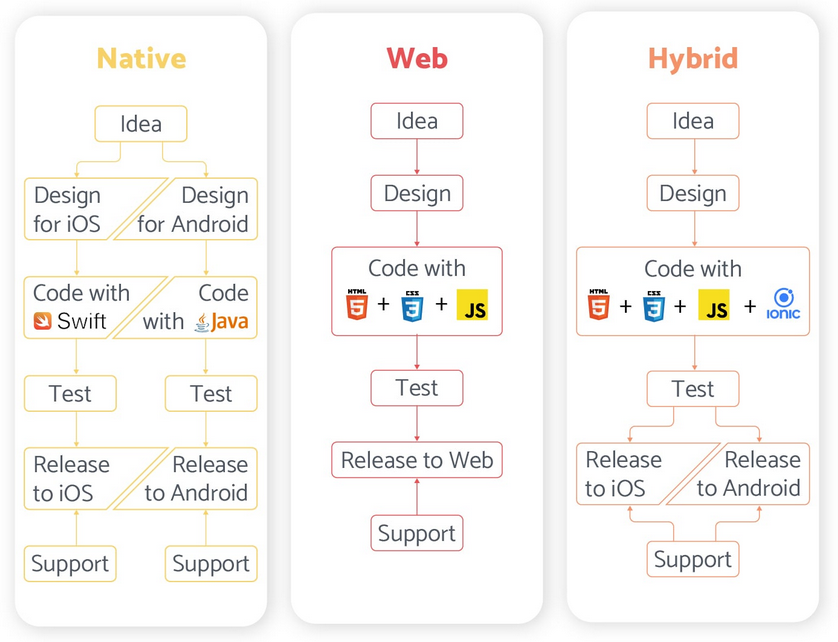
\includegraphics[height=0.4\textheight]{NativeWebHybrid2.png}
    \caption{Native vs Web vs Hybride applicaties \parencite{Merenych2021}.}
    \label{fig:NativeWebHybride}
\end{figure}
Op de figuur is een mooi overzicht te zien van hoe dat de verschillende 
soorten applicaties werken. Elke soort applicatie heeft een andere manier waarop dat ze 
op een platform geïmplementeerd worden.

\section{Native ontwikkeling}
\subsection{Wat is native ontwikkeling?}\label{subsec:wat-is-native-ontwikkeling}
Native ontwikkeling is het proces om native \ref{ch:native-applicaties} applicaties te maken 
voor een specifiek besturingssysteem, zoals Android of IOS. Hierbij wordt er gebruik gemaakt van de 
bijhorende programmeertalen en ontwikkelingsomgevingen die door de platformen worden aangeboden 
\autocite{Meirelles2019}. Ook kunnen ontwikkelaars zoals eerder gezegd gebruik maken van 
platform specifieke APIs die toegang verlenen tot de camera, gps, versnellingsmeter, kompas, 
lijst van contacten, enz...

\subsection{Voordelen van native ontwikkeling}
\paragraph{Schaalbaarheid}
Dankzij de flexibiliteit bij het ontwikkelen van native applicaties en het scheiden van 
de ontwikkeling er van, zijn native applicaties zeer schaalbaar \autocite{Koffer2023}. 
Ook hebben ontwikkelaars de mogelijkheid om elk platform individueel te schalen \autocite{Sakovich2023}. 

\subsection{Nadelen van native ontwikkeling}
\paragraph{Ontwikkelingsteams}
Nog een andere reden van de hoge kost of onderhoudsprijs bij native mobiele applicaties 
zullen de ontwikkelingsteams zijn. Bij het ontwikkeling van een applicatie voor beide 
platformen, zal er gewerkt moeten worden met ofwel één team met de kennis om voor beide 
platformen te ontwikkelen. Of er zal met twee teams gewerkt worden die elk een applicatie 
voor één platform maken \autocite{Kotlin2023}.

\paragraph{Onderhoudstijd}
Na het ontwikkelen van een native applicatie kan het zijn dat er wijzigingen komen of 
dat er updates moeten gebeuren. Aangezien dat er niet wordt gewerkt met één centraal codebase, maar 
met twee onafhankelijke projecten, zullen de wijzigingen of updates op beide projecten 
uitgevoerd moeten worden \autocite{Kotlin2023}.

\subsection{Programmeertalen en frameworks voor native ontwikkeling}
Zoals reeds hebben besproken, gaat native ontwikkeling een applicatie ontwikkelen 
specifiek voor één besturingssysteem. Om die 
applicatie kunnen verscheidene programmeertalen, frameworks 
en \acrshort{ide} gebruikt worden. Deze zijn allemaal specifiek voor ofwel Android of IOS. In de volgende 
secties worden enkele programmeertalen overlopen die gebruikt kunnen worden om het onderzoek uit te voeren.

\subsubsection{Android programmeertalen}
\paragraph{Java}
Java is een all-round programmeertaal met meerdere doeleinden. Eén van die doeleinden 
onder andere is Android applicatie ontwikkeling. Het was de eerste officiële programmeertaal 
voor Android applicatie ontwikkeling. Maar het blijft vandaag de dag nog steeds de 
meestgebruikte \autocite{harkiran2022}. Aangezien het de meestgebruikte programmeertaal 
is, is het soms gemakkelijker om mee te werken aangezien eventuele bugs meestal al zijn 
opgelost door de community \autocite{Thorndyke2021}. Dat wil wel niet zeggen dat het een 
gemakkelijke programmeertaal is om mee te werken. Java kan soms zeer complex zijn waardoor 
onervaren ontwikkelaars het lastig kunnen krijgen \autocite{Kesavan2021}. Daarnaast is Java 
mede door zijn complexiteit een zeer robuust programma dat een heleboel voordelen met zich 
meebrengt zoals: flexibiliteit, portabiliteit en herbruikbaarheid \autocite{Kesavan2021}.

\paragraph{Kotlin}
Momenteel is Kotlin de officiële programmeertaal voor Android applicatie ontwikkeling. 
Het is ontwikkeld door Google en \Gls{JetBrains} als lichtere en meer gebruiksvriendelijke
manier om Android applicaties te maken \autocite{Thorndyke2021}. In vergelijking met Java 
is er geen nood aan puntkomma's en is er minder code nodig om dezelfde applicatie te maken. Daarnaast laat Kotlin 
laat toe om variabelen te maken zonder ze op voorhand te moeten definiëren \autocite{Thorndyke2021}. 
Het wordt door veel bedrijven gebruikt omwille van de herbruikbaarheid van code alsook het 
gebruik van externe \gls{library} \autocite{Kesavan2021}.

\paragraph{C++}
C++ is een alternatieve methode voor Android applicatie ontwikkeling. Om C++ te gebruiken 
moet de \acrshort{andk} gebruikt worden. De applicatie kan wel niet compleet 
met C++ worden gemaakt, maar C++ en de ANDK kunnen gebruikt worden om libraries te ontwikkelen 
waarvan een applicatie gebruik maakt \autocite{harkiran2022}. Het gebruik van C++ voor libraries wordt 
vaak gedaan voor de performantie die C++ met zich meebrengt. Er moet wel rekening worden 
gehouden dat het een moeilijke programmeertaal is om te leren en dus niet voor iedereen weggelegd is 
\autocite{Designveloper2022}.

\paragraph{C\#}\label{pa:csharp}
Origineel is C\# ontwikkeld als object-georiënteerde programmeertaal, dat gebruikt zou 
worden voor desktop, mobiele en web applicaties te maken. Het was een taal die voortkwam 
vanuit C en werd ontwikkeld door Microsoft \autocite{Designveloper2022}. Het is niet alleen 
omdat het al 20 jaar bestaat, dat het daarom een populaire keuze is voor ontwikkelaars 
maar C\# heeft toegang tot het .NET framework \autocite{Kesavan2021}. Het .NET framework 
bied heel wat tools en libraries aan die helpen bij het ontwikkelen van Android applicaties. 
Daarnaast heeft C\# nog een aantal andere voordelen. C\# heeft wat cross-platform 
capaciteiten, waardoor er code overheen platformen gedeeld kan worden en er is een 
\gls{GarbageCollector}, die ervoor zorgt dat er geen geheugen lekken zijn \autocite{Patel2023}.

\paragraph{Dart}
Dart is een open-source programmeertaal, gemaakt door Google dat werd ontworpen om op 
Android platformen te runnen \autocite{Kesavan2021} met de bedoeling van klanten een 
geoptimaliseerde manier te geven om snel applicaties op het Android platform te krijgen 
\autocite{harkiran2022}. Dit wordt gedaan door te focussen op UI development. De wijzigingen 
worden snel aan de ontwikkelaar getoond dankzij de hot-reload. Tot slot is Dart ook gekend 
voor hun performantie en de mogelijkheid om te compilen tot ARM en x64 code \autocite{harkiran2022}.

\paragraph{Corona}
Ondanks dat het minder populair is, is Corona zeker geen slechte alternatief. Het is snel 
en makkelijk om te gebruiken met de capaciteiten om de meeste Android applicaties te runnen 
\autocite{Kesavan2021}. Corona is ook geen programmeertaal op zich, maar een development kit 
dat gebruikt kan worden om Android applicaties te maken door gebruik te maken van Lua. Lua is 
een lichte, efficiënte en open-source programmeertaal dat object-georiënteerd, functioneel, 
data-driven, enz. programmeren ondersteund \autocite{Lua2021}. Om met Corona te werken, worden 
er twee operationele modes gebruikt namelijk de Corona Simulator en Corona Native. De Corona 
Simulator wordt gebruikt om applicaties te maken en Corona Native wordt gebruikt om de Lua 
code te integreren met een Android Studio project om applicaties te maken die native 
functionaliteiten gebruiken \autocite{harkiran2022}.

\subsubsection{IOS programmeertalen}
\paragraph{Swift}
Swift wordt niet enkel en alleen meer gebruikt om mobiele applicaties te ontwikkelen. 
Swift wordt ook gebruikt voor besturingssystemen zoals Windows en Linux. Het werd 
ontwikkeld door Apple als een open-source opvolger van alle C gebaseerde programmeertalen 
zoals Objective-C, C++ en C \autocite{Coursera2022}. Er zijn 3 hoofdzakelijke voordelen 
waardoor Swift zeer populair is geworden bij ontwikkelaars: snelheid, veiligheid en 
introductie niveau \autocite{yuvraj2022}. Als opvolger van alle C gebaseerde programmeertalen, 
heeft het ook een betere performantie bij het uitvoeren van de meeste taken. Daarnaast kunnen 
variabelen ook aangemaakt worden zonder op voorhand een type te definiëren en puntkomma's 
zijn niet verplicht \autocite{Thorndyke2021}.

\paragraph{C\#}
Net zoals bij Android kan C\# ook gebruikt worden om IOS applicaties te ontwikkelen. 
En zoals eerder gezegd, is C\# een object-georiënteerde programmeertaal dat geïntegreerd 
is met het .NET framework \ref{pa:csharp} \autocite{yuvraj2022}. Doorheen de jaren sinds 
2000 wanneer C\# beschikbaar was heeft het heel wat populariteit gewonnen dankzij de 
eenvoudige en hoogwaardige architectuur \autocite{yuvraj2022}. Momenteel is C\# gerankt 
als de 7 populairste programmeertaal \autocite{Johns2023}. C\# gebruikt niet alleen de 
tools en libraries dat .NET te bieden heeft, maar het maakt ook gebruik van de .NET runtime 
omgeving \autocite{Pruciak2022}.

\paragraph{Objective-C}
Objective-C was de originele programmeertaal voor Apple en de fundering van MacOS en 
IOS \autocite{Johns2023}. Het is een \gls{superset} van C, het breid C dus uit en het 
voegt nieuwe functionaliteiten eraan toe \autocite{Johns2023}. Net zoals C\# is Objective-C 
een object-georiënteerde programmeertaal \autocite{Pruciak2022}. Daarnaast bestaat 
het wel al langer dan C\#, Objective-C is ontwikkeld in de vroege 1980's \autocite{Pruciak2022}. 
Aangezien het van C komt, is het ook mogelijk om C code in een Objective-C klasse toe 
te voegen. Daardoor worden Objective-C klassen simpeler, flexibeler en meer schaalbaar 
voor mobiele applicaties \autocite{yuvraj2022}. Dankzij de eenvoud en betere runtijd is 
Objective-C een van de meest gekozen programmeertalen, vooral dankzij de krachtige \acrshort{sdk} 
die worden gebruikt.

\subsection{Tools en IDEs voor native ontwikkeling}
\paragraph{Android Studio}
Android Studio is een populaire IDE die vaak wordt gebruikt in combinatie met 
Kotlin om native Android applicaties te ontwikkelen. Het wordt vaak door ontwikkelaars 
gebruikt omwille van de ingebouwde \gls{emulator} die Android Studio bevat. Hiermee 
kunnen ontwikkelaars verschillende apparaten met verschillende Android versies uit 
testen \autocite{Medewar2022}. Daarnaast ondersteunt de emulator ook verschillende 
features die normaal enkel toegankelijk zijn bij fysieke apparaten, zoals toegang tot 
de camera, locatie, batterij instellingen, enz. \autocite{Okeke2022}. Tot slot biedt 
Android Studio ook een krachtige manier om layouts te maken. Ontwikkelaars kunnen met 
een visuele design editor schermen opbouwen in plaats van code te schrijven, die schermen 
worden dan automatisch door Android Studio omgezet naar xml bestanden \autocite{Medewar2022}. 
Het ondersteund ook GitHub integratie om makkelijk aan grote projecten te werken \autocite{Studio2023}.

\paragraph{Eclipse}
Eclipse is ontwikkeld in 2001 als een Java IDE. Maar over de jaren is het uitgegroeid 
tot een IDE dat meerdere programmeertalen ondersteund \autocite{Medewar2022}. Ondanks 
de ondersteuning van meerdere programmeertalen wordt het nog altijd vaak gebruikt om native 
Android applicaties te ontwikkelen. Het laat ook net zoals Android Studio ontwikkelaars toe 
om makkelijk te werken aan projecten dankzij de GitHub integratie \autocite{Okeke2022}, maar 
het ondersteund ook andere integratiemethoden zoals Maven \autocite{Medewar2022}. Tot slot 
bestaat er dankzij de populariteit een grootte community rondom Eclipse dat meewerkt aan de 
verbetering ervan \autocite{Medewar2022}.

\paragraph{Xcode}
Xcode is een IDE dat wordt gebruikt om software en applicaties te maken voor IOS, macOS, 
iPadOS, watchOS en tvOS \autocite{jahnavisarora2020}. Net zoals bij Android Studio en 
Eclipse bevat ook Xcode een Source Control menu waarmee ontwikkelaars makkelijk met GitHub 
kunnen werken \autocite{Medewar2022}. Om software voor alle Apple gerelateerde besturingssystemen 
te schrijven wordt er gebruik gemaakt van Swift, C, C++ en Objective C compilers 
\autocite{jahnavisarora2020}. Wat Xcode zo populair maakt is de geïntegreerde workflow 
voor coderen, testen, debuggen en ontwerpen van gebruikersinterfaces \autocite{jahnavisarora2020}.

% https://raygun.com/blog/native-app-development/
% https://fireart.studio/blog/android-vs-ios-development/
\paragraph{Samenvatting native ontwikkelomgeving}
Omdat dit onderzoek vooral focust op het verschil tussen native en cross-platform en niet 
de verschillen tussen de native platformen wordt er langs de native kant één platform gekozen.
%foto
Op de foto is duidelijk te zien dat Android het grootste marktaandeel heeft bij mobiele 
applicaties. Daarom wordt Android gekozen als platform voor het uitvoeren van het onderzoek.
\\\\
Om de functionaliteiten van native Android applicaties 
te testen wordt er gebruik gemaakt van de officiële programmeertaal van Android applicaties, 
namelijk Kotlin. Dit zullen we doen omdat Kotlin ontworpen is om veiliger te zijn dan 
sommige andere programmeertalen \autocite{Kesavan2021}, waardoor de kans op bugs en 
fouten kleiner is. Daarnaast is Kotlin makkelijk te integreren in bestaande 
Java-projecten \autocite{Kesavan2021}. Dit bespaart tijd en verhoogt de efficiëntie 
van de ontwikkeling. Tot slot heeft Kotlin een actieve gemeenschap van ontwikkelaars 
die regelmatig updates en nieuwe functies uitbrengen, waardoor de taal zich snel blijft 
ontwikkelen en verbeteren \autocite{Patel2023}.
\\\\
De gebruikte IDE om applicaties te ontwikkelen is Android Studio. Bij Android Studio wordt 
Kotlin standaard ondersteunt terwijl dit bij Eclipse niet het geval is. Daarnaast wordt Kotlin 
door Google aangeraden aan ontwikkelaars \autocite{Medewar2022}.

\section{Cross-platform ontwikkeling}
\subsection{Wat is cross-platform ontwikkeling?}
Cross-platform ontwikkeling is het proces om native applicaties \ref{ch:native-applicaties} 
te maken voor een specifiek besturingssysteem, zoals Android en IOS. Cross-platform wordt 
gebruikt om het platform specifiek probleem van native applicaties op te lossen door beide 
applicaties te ontwikkelen vanuit één codebase \autocite{Khan2021}.

\subsection{Voordelen van cross-platform ontwikkeling}
Net zoals bij web applicaties \ref{ch:VoordelenWebApplicaties}, zal ook bij cross-platform 
ontwikkeling de kostprijs van applicaties lager liggen dan bij native ontwikkeling. 
Dit komt omdat er maar één applicatie ontwikkeld moet worden in plaats van twee. Ook zullen de 
onderhoudskosten lager liggen voor dezelfde reden \autocite{Terekhov2022}. Nog een ander 
groot voordeel van de gedeelde codebase voor twee applicaties is de gedeelde logica ervan. 
Aangezien er maar één codebase is zal de logica voor beide applicaties altijd gelijk zijn, waarbij 
dat bij native ontwikkeling soms niet het geval is \autocite{Kotlin2023}.

\subsection{Nadelen van cross-platform ontwikkeling}
Bij cross-platform ontwikkeling is het niet mogelijk om gebruik te maken van sommige 
functionaliteiten van een apparaat \autocite{Terekhov2022}. Daarnaast kan native 
ontwikkeling indien een apparaat een nieuwe functionaliteit aanbied hier onmiddellijk gebruik 
van maken in vergelijking met cross-platform dat moet wachten op updates voor cross-platform 
ontwikkeling \autocite{Sakovich22023}.

\subsubsection{Verschil met native ontwikkeling}
Het grootste verschil met native ontwikkeling is dat er bij cross-platform maar één 
programmeertaal en IDE nodig is om mobiele applicaties voor zowel Android als IOS te 
ontwikkelen \autocite{Hu2021}. Bij native ontwikkeling is er voor elk platform een 
programmeertaal en IDE nodig. 

\subsection{Frameworks voor cross-platform ontwikkeling}
Om cross-platform te ontwikkelen kunnen verschillende frameworks en 
IDEs gebruikt worden. In de volgende secties worden enkele overlopen die gebruikt kunnen worden  
om het onderzoek uit te voeren.

\paragraph{Flutter}
Flutter is een open-source framework ontwikkeld door Google dat de ontwikkeling toelaat 
van niet alleen Android en IOS applicaties, maar ook Linux, macOS, Fuchsia en Windows 
vanuit één codebase \autocite{Okeke2022a}. Het is vooral populair bij ontwikkelaars 
dankzij de simpelheid om te gebruiken en de performantie \autocite{Sakovich22023}. De 
hoge performantie komt door het gebruik van C en C++ \autocite{Terekhov2022}. Daarnaast 
heeft het ook een \gls{Hotreload} waardoor ontwikkelaars snel resultaten kunnen zien bij 
veranderingen in de code \autocite{Sakovich22023}.

\paragraph{React native}
React native is net zoals Flutter een open-source framework ontwikkeld door Facebook. 
Het laat toe om IOS en Android applicaties te ontwikkelen \autocite{Terekhov2022}. 
Het grootste voordeel van React native is de ontwikkeltijd waarmee applicaties ontwikkeld 
kunnen worden \autocite{Terekhov2022} en de grote community die meehelpt aan het ontwikkelen 
van externe libraries \autocite{Okeke2022a}. Dankzij die externe libraries hebben ontwikkelaars 
toegang tot native features die normaal voor cross-platform ontwikkeling niet toegankelijk is. 
Deze externe libraries kunnen geschreven zijn in Objective-C, Swift of Java \autocite{Okeke2022a}. 
Tot slot heeft React native ook een hot reload functie net zoals flutter waardoor ontwikkelaars 
snel resultaten kunnen zien bij veranderingen in de code \autocite{Terekhov2022}.

\paragraph{.NET MAUI (vroeger Xamarin)}
.NET MAUI is net zoals Flutter en React native een open-source framework ontwikkeld door 
Microsoft. Het maakt gebruik van C\# als programmeertaal en het .NET framework voor 
native libraries \autocite{Sakovich22023}. Net zoals bij Flutter en React native bezit 
ook .NET MAUI over een hot reload functie om snel te kunnen ontwikkelen en debuggen. 
Dankzij het gebruik van C\# bezit ook .NET MAUI net zoals Flutter en React native over 
een hoge performantie \autocite{Okeke2022a}. Een belangrijk nadeel is echter dat 
applicaties niet altijd compatibel zijn met de nieuwste versies van 
Android of iOS \autocite{Terekhov2022}.

\paragraph{Samenvatting frameworks}
%TODO sure
Niet alle frameworks voor cross-platform ontwikkeling worden hier beschreven, maar de drie 
frameworks die hier wel beschreven zijn hebben allemaal een gelijkaardige performantie. React native en 
.NET MAUI hebben ook makkelijk toegang tot native features dankzij de native libraries. 
Uit deze drie frameworks wordt React native gekozen om cross-platform te ontwikkelen 
dankzij de performantie, native libraries en grote community er rond. React native 
bevat voor dit onderzoek de beste eigenschappen om het onderzoek uit te voeren.

\subsection{IDEs voor cross-platform ontwikkeling}
\paragraph{Visual Studio Code}
Er is maar één IDE die eruit springt en dat is Visual Studio Code. Het is een 
universele IDE die gebruikt kan worden voor alle programmeertalen. Daarnaast is er een 
groot aanbod van extensies die het mogelijk maken om de IDE aan te passen aan de 
specifieke behoefte van de ontwikkelaar \autocite{Heller2022}. Daarom wordt Visual 
Studio Code gebruikt als IDE om cross-platform te ontwikkelen.

\section{Functionaliteiten}
\subsection{Keuze te onderzoeken functionaliteiten}
Om een vergelijking te kunnen maken tussen native en cross-platform ontwikkeling, 
zijn er een aantal functionaliteiten nodig om te onderzoeken. 

\paragraph{Basisfunctionaliteiten}
Dit omvat functionaliteiten die elke mobiele applicatie zou moeten hebben. Zoals 
het openen van de app met ondertussen een laadscherm tonen. Daarnaast het navigeren 
tussen verschillende schermen binnen de applicatie. Deze functionaliteiten zijn bij 
elke applicatie aanwezig en vormen dus een belangrijk onderdeel van de gebruikerservaring 
en daarom ook een belangrijk onderdeel van de vergelijking tussen native en cross-platform.
Hierbij zullen we vooral kijken naar het invloed op de opstartsnelheid van de applicatie 
en de snelheid waarmee er genavigeerd kan worden tussen de verschillende schermen.

\paragraph{Audio- en videospelers}
Een mobiele app kan verschillende soorten media afspelen, zoals video's en muziek. 
Hierbij zullen we kijken naar de implementatie van deze functionaliteit in 
zowel native als cross-platform ontwikkeling. We zullen de integratie van externe bibliotheken 
voor het afspelen van media en video's en hun performantie onderzoeken.

\paragraph{Gebruik van sensoren}
Mobiele apparaten bevatten verschillende sensoren, zoals de accelerometer en gyroscoop. 
Ze kunnen worden gebruikt in mobiele applicaties om bijvoorbeeld beweging te detecteren 
of de oriëntatie van het apparaat. Bij het gebruik van sensoren kijken we naar hoe deze 
sensoren geïmplementeerd kunnen worden en de snelheid waarmee data ingelezen kan worden 
in zowel native als cross-platform ontwikkeling.

\paragraph{Notificaties}
Notificaties (meldingen) zijn berichten die worden weergegeven op het scherm van een 
apparaat. Ze kunnen komen via het internet of door een applicatie zelf. We zullen hierbij 
kijken naar de implementatie van enkel lokale notificaties. Aangezien de performantie van 
push-notificaties gedeeltelijk zal afhangen van een extern framework of netwerk waarover 
dezelfde performantie niet gegarandeerd kan worden.

% %\paragraph{Locatie}
% %\paragraph{func7}
% %\paragraph{func8}
% %\paragraph{func9}
% %\paragraph{func10}

\section{Samenvatting stand van zaken}
Nu dat er een inzicht verkregen is in mobiele applicaties en de ontwikkeling ervan, 
kan het onderzoek van start gaan. Alle functionaliteiten worden voor 
zowel native als cross-platform ontwikkeld. Bij native ontwikkeling wordt 
Kotlin en Android Studio gebruikt om native applicaties te maken. 
Bij cross-platform wordt React-native en Visual Studio Code gebruikt om de 
native applicaties te maken.














